\documentclass[]{tufte-book} %justified ovverides the rugged-right style


\usepackage{color}
\usepackage{enumitem}
\usepackage{framed}
\usepackage{graphicx}
\usepackage{listings}
\usepackage{xcolor}

\usepackage{multicol}              
\usepackage{multirow}
\usepackage{booktabs} 

\usepackage[]{hyperref}
\definecolor{darkblue}{rgb}{0,0,.5}
\hypersetup{colorlinks=true, breaklinks=true, linkcolor=darkblue, menucolor=darkblue, urlcolor=darkblue, citecolor=darkblue}
  
\usepackage[toc,page]{appendix}

\setcounter{secnumdepth}{1}
\setcounter{tocdepth}{1}

\lstset{
language=[LaTeX]{TeX},
breaklines = true,
breakautoindent = false,
breakindent = 0pt,
commentstyle=\color{gray},
frame=single,
framerule=0.4pt,
framesep=3pt,
xleftmargin=3.4pt,
xrightmargin=3.4pt,
basicstyle=\normalfont\scriptsize,
keywordstyle=\color{blue}\sffamily,                                
identifierstyle=\color{black},
numbers=none, 
morekeywords = {maketitle, tableofcontents, subsection, 
				citet, cite, citep, bottomrule, toprule,
				midrule, addlinespace, includegraphics, 
				bibpunct, definecolor, hypersetup}  
}



\lstdefinelanguage{BibTeX}
{keywords={%
		@article,@book,@collectedbook,@conference,@electronic,@ieeetranbstctl,%
		@inbook,@incollectedbook,@incollection,@injournal,@inproceedings,%
		@manual,@mastersthesis,@misc,@patent,@periodical,@phdthesis,@preamble,%
		@proceedings,@standard,@string,@techreport,@unpublished%
	},
	comment=[l][\itshape]{@comment},
	sensitive=false,
}


\title{Scientific writing\\with LaTeX}
\author{MSc Module Research Skills}



\begin{document}
\let\cleardoublepage\clearpage
\maketitle

\thispagestyle{empty}
\null


\begin{fullwidth}
These lecture notes are part of the course material for the MSc module Research Skills (website \href{http://florianhartig.github.io/ResearchSkills/}{here}). First edition 2015, this version was created \today.\\[0.5cm]
\end{fullwidth}

\begin{fullwidth}
\href{http://www.uni-regensburg.de/biologie-vorklinische-medizin/theoretische-oekologie/mitarbeiter/hartig/index.html}{Florian Hartig}\\
University of Regensburg
Germany\\[0.2cm]
If you find typos or have suggestions, please report them by creating a ticket \href{https://github.com/florianhartig/ResearchSkills/issues}{here}

\end{fullwidth}


\vfill
\begin{fullwidth}
These notes were created 2014 by Paul Bauche based on the existing RS LaTeX exercise of FH. Updates 2015 by Severin Hauenstein and Florian Hartig. This work is licensed under a Creative Commons Attribution-NonCommercial-NoDerivatives 4.0 International License.
\end{fullwidth}

\tableofcontents

\chapter{Introduction}

This tutorial will help you start working with \LaTeX. You will learn how to set up a basic  \LaTeX document which contains all the elements typically used in a scientific article, for example references, graphics, tables or formulae. 

 \LaTeX\ is a script-based typesetting program which allows you to set the design of your report, article, book or whatever written statement via written commands. This may appear a bit cryptic in the beginning, but after a short time of getting used to this way of working you will realize how much time you can save and how much nicer and more professional your documents look.

 Basically, when it comes to typesetting software there are two distinguishable types. The first and most common is called \emph{"What You See Is What You Get"} (WYSIWYG). This describes software such as OpenOffice Writer, Microsoft Word etc. where you can see how your document is going to look in the end while you are working on it, but it might be difficult to create a document exactly the way you wanted it to be. The second type is called \emph{"What You Get Is What You Want"}(WYGIWYW). This is the category \LaTeX\ belongs to. It means that while you are working on your document you do not get a visual representation of the final result, but your final result will be the way you imagined it when you started.  	

\paragraph{Templates}
Since the basic structure of \LaTeX\ documents of the same class is similar in most cases, you may save some time by using existing templates. Prof. Dormann created such a template for a Master's thesis. It is available \href{https://github.com/florianhartig/ResearchSkills/tree/master/Labs/LaTeX/LaTeX_Templates/Template-BScMSc-Freiburg}{here}.
 
Other templates for the Tufte-style book (book\_1), the Legrand Orange book (book\_2) or some stylish article (article\_3) can be found \href{https://github.com/florianhartig/ResearchSkills/tree/master/Labs/LaTeX/LaTeX_Templates/LatexTemplates}{here}.
 
The \href{https://github.com/florianhartig/ResearchSkills/tree/master/Labs/LaTeX/Practical}{\LaTeX\ document we use for the \LaTeX\ practical} of this course can also be used as template for a simple article. 

\chapter{Setting up \LaTeX\ on your computer}

First you need to set up \LaTeX\ on your computer. Basically, a \LaTeX\ system consists of two components: a \LaTeX\ distribution, and an editor.

\paragraph{Distribution -}There are different distributions, also depending on your operating system. For Windows, the clear choice is MikTex. For Mac, MacTeX is probably the best choice, but there are other options as well. The \LaTeX\ distribution under Linux is called TeX Live and can be installed through the package managers of all major distributions.

\paragraph{Editor -}The second thing you need is an editor. In principle you can use any editor (\LaTeX\ documents are just text files), but it is more convenient to use a specialised \LaTeX\  editor that is already set up to work together with your \LaTeX\ distribution. \marginnote{Texmaker and TeXstudio are very similar (TeXStudio originated from a previous version of TeXmaker). TeXstudio is a bit more automatized and offers more buttons.} We recommend using one of the free \LaTeX\ editors TexMaker or TexStudio, and some of the comments later in this document will assume that you will be working with a MikTex / TexMaker or TeXstudio combination (Most of the advice, however, as well as any proper \LaTeX\ document, can be used on any system).

To get MikTex and TexMaker or TeXstudio, search for it on the web, then download and install it on your computer. Make sure you install from the project website and not from third-party sites that often offer pretty old versions. 
  
Before you start your project you have to keep a couple of things in mind that will later on help you to keep track of what you are doing and to avoid unnecessary errors.
 
If you use MikTex, it is helpful to be connected to the internet in some way to enable \LaTeX\ to download packages on the fly.\marginnote{If you install MacTex, choose the full installation because missing packages are not installed automatically.} For other distributions, you will have to install missing packages by hand. 


\chapter{Starting a new \LaTeX\ project}


\section{Creating a new directory for the project}

First of all, create a folder on your computer and make sure that you have the necessary\marginnote{Always create a new project folder with a distinct name when starting a \LaTeX\ document!} rights to read and write in that location. Do not simply start your project on the desktop since \LaTeX\ creates additional files as you compile your project and you will make a mess of things.
 
When creating the folder and all following files make sure you do not use spaces or\marginnote{No spaces or special symbols in file or folder names anywhere in your file path!} special symbols. Nowhere in the path to your files should be any of those symbols. Stick to letters, numbers and underscores. 


\section{Preparing your editor}

In TexMaker you have several options to configure the user interface. The most important ones shall be explained briefly. 

It is advisable to set the spell check to the language you want to write your article in. You can do that under "Options -> Configure TexMaker -> Editor -> Spelling Dictionary". The most common languages are already part of your software and you can just choose the one you need.  

Here you can also choose the text encoding of your editor. It is recommended to use UTF-8.

Under "Options -> Interface Language" you can choose the language for TexMaker. This does not affect the spell check but is solely for your convenience.  


\section{Creating a \LaTeX\ document}

Now that you have created your project folder, you can create your first \LaTeX\ document. Navigate to your project folder and create a new text file. Open this file and type the following line:\\[5pt]

\emph{\% This is my first Latex document. There are many documents like it, but this one is mine.}\\[5pt]

Make sure you do not forget the percent symbol \%. Then save your document as \verb!my_first_article.tex! and close the editor. With the extension .tex you make sure that your system recognizes the file as a \LaTeX\ document.\marginnote{The \% symbol is used for comments, lines of text that are not interpreted by \LaTeX!}
Now open \verb!my_first_article.tex! with your \LaTeX\ editor (e.g. Texmaker). You will notice that the line you wrote now looks gray.\\[5pt]

\begin{lstlisting}
% This is my first Latex document. There are many documents like it, but this one is mine.
\end{lstlisting}

The gray color symbolizes a \emph{comment}. The comment is declared by using the \% symbol at the start of the line. Everything written after the \% is not interpreted by \LaTeX\ and does not appear in your document. Comments can be used to structure your document for yourself and others using it. You can explain functions and why you include packages. This is especially useful if you want to reuse the structure of our document again for other papers.    

\chapter{Start editing your document}

To start your actual document, you first need to declare the type of document you want to create. This is done in the so called "preamble" of the \LaTeX\ document. There you can also declare additional options and include packages to increase the functionality of \LaTeX.

For the purpose of this tutorial you are going to create a scientific article. This type of document is declared by \verb!\documentclass{article}!. This defines a few design characteristics such as line spacing and the width of the borders of the page for your document. The backslash \verb!\! is used to indicate to \LaTeX\ that the following is a command. In \LaTeX\, commands are used for everything from setting your font type to including pictures or graphics.  

Now you can begin with your document.\marginnote{Every \emph{begin} statement requires an \emph{end} statement!} To do so, you start with the line \verb!\begin{document}!.
This should result in two lines being created: in addition to \verb!\begin{document}! there should also be a line saying \verb!\end{document}!. If this is not the case, just type it yourself. Now  you should have a document looking like this:\\[5pt]


\begin{lstlisting}
% This is my first Latex document. There are many documents like it, but this one is mine.

\documentclass{article}

\begin{document}

\end{document}
\end{lstlisting}


This is the most basic setup for your document. To start adding some text, you can now write a few lines between the begin- and end-document statements. Since this is supposed to be a scientific article, it should start with an abstract. The abstract is also framed by a begin- and an end-statement. They are \verb!\begin{abstract}! and \verb!\end{abstract}!. For your abstract try:\\[5pt] 

\textit{This is my first \LaTeX\ document. I am going to learn a lot about typesetting and writing articles in \LaTeX.}\\[5pt]


Now your document should look like this:\\[5pt]


\begin{lstlisting}
% This is my first Latex document. There are many documents like it, but this one is mine.

\documentclass{article}

\begin{document}

\begin{abstract}
This is my first \LaTeX\ document. I am going to learn a lot about typesetting and writing articles in \LaTeX\ and my papers will look really nice from now on.
\end{abstract}

\end{document}
\end{lstlisting}


You should now be able to compile your document and create a pdf file from it. To do so, you just have to press compile in your \LaTeX\ editor. You should notice the  \LaTeX\ symbol. This was created by using the \verb!\LaTeX! command. After the abstract you can start your first section. This is usually the introduction. You can add sections via \verb!\section{}!. Here no begin- or end-statement is needed. One section lasts until the next one starts or the document ends. To add the section "Introduction" to your document, now type  \verb!\section{Introduction}! below \verb!\end{abstract}! in your document and write a few lines like\\

\begin{lstlisting}

This is my \textbf{first} \emph{sentence}.

This is my \textit{second} sentence. 

This is my third sentence. You can also put some distance between lines.\\[3mm]
Test 

\end{lstlisting}

Now your document should look like this:\\[5pt]

\begin{lstlisting}
% This is my first Latex document. There are many documents like it, but this one is mine.

\documentclass{article}

\begin{document}
\begin{abstract}
This is my first \LaTeX\ document. I am going to learn a lot about typesetting and writing articles in \LaTeX! and my papers will look really nice from now on.
\end{abstract}

\section{Introduction}

This is my \textbf{first} \emph{sentence}.

This is my \textit{second} sentence. 

This is my third sentence. You can also put some distance between lines.\\[3mm]
Test 

\end{document}
\end{lstlisting}

Compile your document to notice the effect of the new commands. \verb!\textbf{}! leads to \textbf{bold} fonts, \verb!\textit{}! leads to \textit{italic} fonts, and \verb!\emph{}! \emph{emphasizes} what ever you put into the curly brackets. Additionally, you learned two ways to add a line break to your document. The first one is to simply leave a blank line after the point at which you want to break the line. This also leads to an indent at the beginning of the next line, which makes for better readability. The second one is to add \verb!\\!. This method can be refined by adding the exact spacing either in mm, pt or relative to the default line height in square brackets, for example \verb!\\[3mm]!. No indent follows this type of line break. 

\chapter{The preamble}

As mentioned before, every \LaTeX\ document must have a preamble.\marginnote{In the preamble, you can include new packages and set general parameters and metadata for your document!} The preamble is everything you write before the \verb!\begin{document}! statement. Here you declare the packages you want to use, define styles, and you can add some metadata to your document, such as the author or the title of your article. These two are added by using the \verb!\author{}! and \verb!\title{}! commands. Add them to your document right below the \verb!\documentclass{}! command, write a title in the curly brackets after \verb!\title! and your name in the curly brackets after \verb!\author! and compile again. There should be no noticeable difference. Now right under the \verb!\begin{document}! statement add \verb!\maketitle! and compile again. Your pdf document should now have a title, your name and the current date at the top. The \verb!\maketitle! command uses the information you provided in the preamble to create a title for your article. If everything worked, your \LaTeX\ document should now look like this:\\[5pt]


\begin{lstlisting}
% This is my first Latex document. There are many documents like it, but this one is mine.

\documentclass{article}
\author{FirstName LastName}
\title{My first \LaTeX\ document}

\begin{document}
\maketitle

\begin{abstract}
\noindent This is my first \LaTeX\ document. I am going to learn a lot about typesetting and writing articles in \LaTeX\ and my papers will look really nice from now on.
\end{abstract}

\section{Introduction}
This is my \textbf{first} \emph{sentence}.

This is my \textit{second} sentence. 

This is my third sentence. You can also put some distance between lines.\\[3mm]
Test 

\end{document} 
\end{lstlisting}


\chapter{Equations in \LaTeX}

Here you will learn how to write equations in \LaTeX. There are two basic types of equations. First, there are inline equations which can be used to write down basic mathematical expressions and equations like $\alpha = 3.5$. or $\lambda = \sqrt{\alpha}$ within your text. Second are the numbered equations. They will appear separated from your text like this:

\begin{lstlisting}
\begin{equation} 
\lambda = \int_{m_0}^\infty f(\Theta) d \Theta 
\end{equation}
\end{lstlisting}

They will be numbered (in this case as the first equation in chapter six), which allows you to easily reference the equation later on in your text. You can use this to write down more complex equations or expressions. As an exercise, you can now create those two types within your own document and put them in a new section named "Equations". You will start with an inline equation. An inline equation is surrounded by \$ symbols to separate it from the rest of the text. For this purpose, start a new subsection called "Inline Equations". A subsection can be created with the \verb!\subsection{}! command. Your first inline equations will be \verb!$\alpha = 3.5$! and \verb!$\lambda = \sqrt{\alpha}$!. To emphasize the inline effect, put a short sentence before the equation. As you can see, Greek letters can be written by typing a \verb!\! before the full name of the letter. Additionally the \verb!\sqrt{}! command is used for the square root symbol. Include this section in your document:\\[5pt]   


\begin{lstlisting}
\subsection{Inline equations}
This is our first inline equation $\alpha = 3.5$. $\lambda = \sqrt{\alpha}$. 

\end{document}  
\end{lstlisting}

Next come your numbered equations. A numbered equation starts with the \verb!\begin{equation}! statement and ends with \verb!\end{equation}!. In between you can\marginnote{Use inline equations for short expressions and numbered equations for more complex equations!} put text as well as all the statements used in equations. Try it yourself now. Start a new subsection called "Numbered Equations" and write down a short sentence followed by:\\ \verb!\begin{equation}! \\ \verb!m = \left( \frac{a \cdot b}{c} \right)! \\ \verb!\end{equation}! \\ and another short sentence followed by:\\ \verb!\begin{equation}\!\\ \verb!\lambda = \int_{m_0}^\infty f(\Theta) d \Theta!\\ \verb!\end{equation}!.\\
Include this section in your document:\\[5pt]

\begin{lstlisting}

\subsection{Numbered equations}
This is our first numbered equation.

\begin{equation}
m = \left( \frac{a \cdot b}{c} \right)
\end{equation}
 
This is our second numbered equation.
 
\begin{equation} 
\lambda = \int_{m_0}^\infty f(\Theta) d \Theta 
\end{equation}
\end{lstlisting}

Your document should now look like this:\\[5pt]


\begin{lstlisting}
% This is my first Latex document. There are many documents like it, but this one is mine.

\documentclass{article}
\author{FirstName LastName}
\title{My first \LaTeX\ document}

\begin{document}
\maketitle

\begin{abstract}
This is my first \LaTeX! document. I am going to learn a lot about typesetting and writing articles in \LaTeX! and my papers will look really nice from now on.
\end{abstract}

\section{Introduction}
This is my \textbf{first} \emph{sentence}.

This is my \textit{second} sentence.

This is my third sentence. You can also put some distance between lines.\\[3mm]
Test 

\section{Doing equations}

\subsection{Inline equations}
This is our first inline equation $\alpha = 3.5$. $\lambda = \sqrt{\alpha}$. 

\subsection{Numbered equations}
This is our first numbered equation.

\begin{equation}
m = \left( \frac{a \cdot b}{c} \right)
\end{equation}
 
This is our second numbered equation.
 
\begin{equation} 
\lambda = \int_{m_0}^\infty f(\Theta) d \Theta 
\end{equation}

\end{document} 
\end{lstlisting}


As you can see, there are a lot of new symbols added, but if you look at them, they are pretty self explanatory. \verb!\infty! is used for the infinity symbol $\infty$ , \verb!\frac{}{}! is used for fractions such as $\frac{x}{y}$ and \verb!\cdot! is used for the multiplication dot $\cdot$. A bit more complicated is \verb!\int!, which is used for integrals. The lower bound is indicated by an underscore " \_ " and the upper bound by the  \^. The full expression for an integral is \verb!\int_x^y! which then looks like $\int_x^y$. Brackets can be placed with the commands \verb!\left(! and \verb!\right)!. 

\chapter{Labels and referencing}

When adding graphs, tables, pictures or equations to your document,\marginnote{Labels and references are important for you and for others to easily link written information to graphic content!} it is common to number these and refer to the number in the text to allow the reader to easily connect your text to the respective visualization. In addition, you might also want to number sections to be able to later refer to them. The numbering is done automatically by \LaTeX\ for all these types. To reference them in your document you just need to label them. The commands used for this purpose are \verb!\label{}! and \verb!\ref{}!. You assign a specific label to the object you want to reference later on by simply placing \verb!\label{}! behind the object you want to reference. Here it is common to use a short prefix to indicate the type of object you want to label such as \emph{sec} for sections, \emph{fig} for figures, \emph{tab} for tables\marginnote{Use abbreviated prefixes to quickly identify your labels!} and so on. This makes it easy to distinguish between different objects connected to the same topic (e.g. a graph and a table displaying the same kind of data). You can also make your references interactive. This means you can link your references to the actual content to make navigating the pdf even easier. To do so you need to include the \emph{hyperref} package in your document preamble. You can then use the \verb!\hypersetup! command to define the formatting of your references. Here we colored them in dark blue. You can use the packages \emph{color} and \emph{xcolor} to increase the spectrum of colors you can use and to enable the definition of custom colors from RGB values. To see how this is done, look at the following:
\marginnote{\emph{hyperref} allows you to create interactive links between your references and the referenced content. This makes navigating large documents a lot easier!}

\begin{lstlisting}
\usepackage[]{hyperref}
\usepackage{color}
\usepackage{xcolor}
\definecolor{darkblue}{rgb}{0,0,.5}
\hypersetup{colorlinks=true, breaklinks=true, 
linkcolor=darkblue, menucolor=darkblue, 
urlcolor=darkblue, citecolor=darkblue}
\end{lstlisting}

As a quick exercise, you are now going to label your numbered equations and the introduction section and reference them in a new section called \emph{Labels and referencing}. Do so by placing a label behind the \verb!\section{}! and the \verb!\begin{equation}! statements. The label you assign here is just for you, to help you distinguish it from the others. The \verb!\ref{}! command only returns the number of the object. To reference your labels simply type \verb!\ref{}! with the label you assigned within the curly brackets. Your document should now look like this:


\begin{lstlisting}
% This is my first Latex document. There are many documents like it, but this one is mine.

\documentclass{article}
\author{FirstName LastName}
\title{My first \LaTeX\ document}

\usepackage[]{hyperref}
\usepackage{color}
\usepackage{xcolor}
\definecolor{darkblue}{rgb}{0,0,.5}
\hypersetup{colorlinks=true, breaklinks=true, 
linkcolor=darkblue, menucolor=darkblue, 
urlcolor=darkblue, citecolor=darkblue}

\begin{document}
\maketitle

\begin{abstract}
This is my first \LaTeX! document. I am going to learn a lot about typesetting and writing articles in \LaTeX! and my papers will look really nice from now on.
\end{abstract}

\section{Introduction}
This is my \textbf{first} \emph{sentence}.

This is my \textit{second} sentence.

This is my third sentence. You can also put some distance between lines.\\[3mm]
Test 

\section{Doing equations} \label{equations}

\subsection{Inline equations}
This is our first inline equation $\alpha = 3.5$. $\lambda = \sqrt{\alpha}$. 

\subsection{Numbered equations}
This is our first numbered equation.

\begin{equation} \label{eq: definition of m}
m = \left( \frac{a \cdot b}{c} \right)
\end{equation}
 
This is our second numbered equation.
 
\begin{equation} \label{eq: definition of lambda}
\lambda = \int_{m_0}^\infty f(\Theta) d \Theta 
\end{equation}!.\\

\section{Labels and referencing}
In LaTeX, everything can be labeled, and after that it can be referenced. Consider for example section~\ref{sec: equations}, where eq.~\ref{eq: definition of lambda} and eq.~\ref{eq: definition of m} are defined.

\end{document}  
\end{lstlisting}


\chapter{Including figures}

As mentioned before, you can also include graphs and pictures in your \LaTeX\ document. This can be done via the \emph{grapicx} package.\marginnote{Remember that you can include packages in the preamble before your \emph{begin document} statement!}
The easiest way to include figures in your document is by placing the file containing your figure (e.g. a PDF or JPG) in your project folder. That way you only need to specify the name of the file when including it and not the full path. You can however place it in another location in your file system or in a subfolder of your project folder and give the file path to \LaTeX\ (but keep in mind not to use spaces or special symbols in your file and path names).

To include images in your \LaTeX\ document, you first need to define a figure space. This can be achieved by using the \verb!\begin{figure}! and \verb!\end{figure}! statements. In between these statements you can now include your image and add a caption to it to briefly summarize what is displayed here. To do so, you need two commands: \verb!\includegraphics[scale=]{}!, with the name or file path of the image to include without the file extension, and \verb!\caption{}!. Most of the time you want your image to be displayed in the center of the lines you are placing it in. For that you can use the command \verb!\centering! one line above the \verb!\includegraphics[scale=]{}! statement.

There should be two image files in your training material, a picture of Albert Einstein in his study and a boxplot graph. Include them into your document. They should be 6 cm wide. 

\begin{lstlisting}
\begin{marginfigure}
\includegraphics[width=6cm]{../example/einstein}
\caption{This photograph by Ferdinand Schmutzer shows Einstein in his study}
\end{marginfigure}
\end{lstlisting}

To include two pictures side by side, just put them into the same figure and make sure to set their width to 3 cm. For each figure, you just need one caption even if it includes several images. And do not forget to label your figures.   

Your document should now look like this:\\[5pt]


\begin{lstlisting}
% This is my first Latex document. There are many documents like it, but this one is mine.

\documentclass{article}

\usepackage{graphicx}

\usepackage[]{hyperref}
\usepackage{color}
\usepackage{xcolor}
\definecolor{darkblue}{rgb}{0,0,.5}
\hypersetup{colorlinks=true, breaklinks=true, 
linkcolor=darkblue, menucolor=darkblue, 
urlcolor=darkblue, citecolor=darkblue}

\author{FirstName LastName}
\title{My first \LaTeX\ document}

\begin{document}
\maketitle

\begin{abstract}
This is my first \LaTeX! document. I am going to learn a lot about typesetting and writing articles in \LaTeX! and my papers will look really nice from now on.
\end{abstract}

\section{Introduction}
This is my \textbf{first} \emph{sentence}.

This is my \textit{second} sentence.

This is my third sentence. You can also put some distance between lines.\\[3mm]
Test 

\section{Doing equations} \label{equations}

\subsection{Inline equations}
This is our first inline equation $\alpha = 3.5$. $\lambda = \sqrt{\alpha}$. 

\subsection{Numbered equations}
This is our first numbered equation.

\begin{equation} \label{eq: definition of m}
m = \left( \frac{a \cdot b}{c} \right)
\end{equation}
 
This is our second numbered equation.
 
\begin{equation} \label{eq: definition of lambda}
\lambda = \int_{m_0}^\infty f(\Theta) d \Theta 
\end{equation}!.\\

\section{Labels and referencing}

In LaTeX, everything can be labeled, and after that it can be referenced. Consider for example section~\ref{sec: equations}, where eq.~\ref{eq: definition of lambda} and eq.~\ref{eq: definition of m} are defined.

\section{Including figures}

\begin{figure}
\centering
\includegraphics[width=6cm]{einstein} % without file extension
\caption{This shows Einstein in his study}\label{fig: einstein}
\end{figure}  

\begin{figure}
\centering
\includegraphics[width=3cm]{einstein}
\includegraphics[width=3cm]{einstein}
\caption{This shows Einstein in his study}\label{fig: einstein2}
\end{figure}  


\begin{figure}
\centering
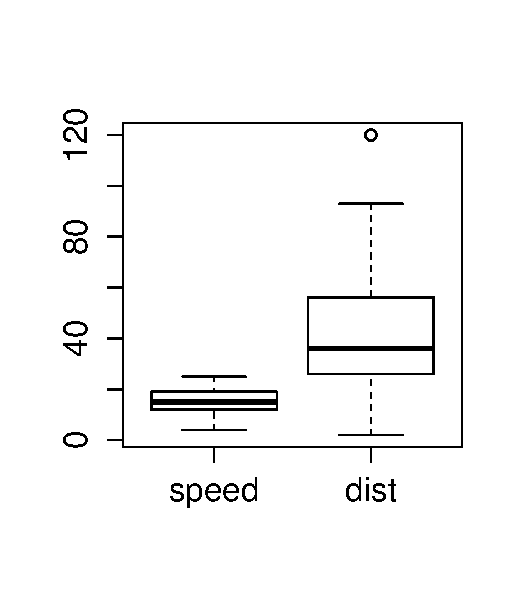
\includegraphics[width=6cm]{boxplot} % without file extension
\caption{This shows a boxplot}\label{fig: boxplot}
\end{figure} 

\end{document}  
\end{lstlisting}


\chapter{Tables}

A very common way of displaying data is to use tables\marginnote{\begin{tabular}{|c|c|}
\hline 
1 & 1 \\ 
\hline 
2 & 1 \\ 
\hline 
\end{tabular}\\[2mm] 

\noindent This is a very simple table created with the \emph{tabular} command!}. 
They are a very efficient way to sort large amounts of data and to make them easy to understand. In \LaTeX\ there are different ways to create and display tables. The easiest way is to use the \verb!\begin{tabular}{}! command. In the curly brackets you can define the number of columns with the following syntax \verb!\begin{tabular}{|c|c|}!. This would for example create a table with two columns and centered text. The columns are later separated by the \& (ampersand) symbol. To add rows you have to break the line with \verb!\\! and optionally add a horizontal line with the \verb!\hline! command. Try to recreate the table on the right and keep in mind that every \emph{begin} statement needs an \emph{end} statement. As you can see, this kind of table is very simplistic and does not look professional or well suited for large amounts of data that require some explanation and additional information. To create proper tables you need additional packages. These packages are called \emph{multicol, multirow} and \emph{booktabs}. Include them in your document now. Look at the following code snippet:

\begin{lstlisting}

\begin{table*}\label{Table: Fit types}
  \centering
  \begin{tabular}{l@{\hspace{0.2cm}}l@{\hspace{0.2cm}}l} \toprule
  \textsc{Case} & \textsc{Explanation} & \textsc{Dimensions} \\ \midrule \addlinespace[0.2cm] 
  \multicolumn{3}{l}{Parameterization to virtual data, 3 PFTs:}  \\
  $V1$ & Data: SDD, GRO, reduced parameters &  $12,96$ \\ 
  $V2$ & Data: SDD, GRO, full parameters &  $26,96$  \\ 
  $V3$ & Data: SDD, reduced parameters &  $12,48$ \\ 
  $V4$ & Data: total SDD, reduced parameters &  $12,16$ \\ 
  $V5$ & Data: BM, reduced parameters &  $12,3$ \\  [0.2cm] 

  \multicolumn{3}{l}{Parameterization to Ecuadorian field data, 7 PFTs:} \\
  $E1$ & Data: SSD  &  $18,112$ \\ \bottomrule \\
\end{tabular}
\caption{Table caption}
\end{table*}

\end{lstlisting} 

As you can see, it is way more complex than the simple table, but it also allows a more informative and more structured table design. You do not need to specify the dimensions of the table in advance. The columns are still separated by the \& symbol The rows are separated simply by a line break. Additionally, the table is divided into different vertical sections which are indicated by the \emph{toprule, midrule} and \emph{bottomrule} statements. These sections can be used to display additional information such as a header for the columns or to aggregate different treatments in one table. The \verb!\multicolumn{}{}{}! \marginnote{use \emph{multicolumn} to aggregate multiple columns into one e.g. for footnotes or headers} command can be used to write over several columns e.g. for table headlines or explanations. The first curly bracket defines the number of columns you want to aggregate, the second one the style ("l" means left-justified) and in the third curly bracket you can put your text. In this case the rows are enclosed in \$ symbols to give them the look of a formula and separate them from the headlines. When compiled correctly the table should look like this:\marginnote{Stick to this kind of table whenever you write a scientific article, report or thesis!} 
\begin{table*}\label{Table: Fit types}
  \begin{tabular}{l@{\hspace{0.2cm}}l@{\hspace{0.2cm}}l} \toprule
  \textsc{Case} & \textsc{Explanation} & \textsc{Dimensions} \\ \midrule \addlinespace[0.2cm] 
  \multicolumn{3}{l}{Parameterization to virtual data, 3 PFTs:}  \\
  $V1$ & Data: SDD, GRO, reduced parameters &  $12,96$ \\ 
  $V2$ & Data: SDD, GRO, full parameters &  $26,96$  \\ 
  $V3$ & Data: SDD, reduced parameters &  $12,48$ \\ 
  $V4$ & Data: total SDD, reduced parameters &  $12,16$ \\ 
  $V5$ & Data: BM, reduced parameters &  $12,3$ \\  [0.2cm] 

  \multicolumn{3}{l}{Parameterization to Ecuadorian field data, 7 PFTs:} \\
  $E1$ & Data: SSD  &  $18,112$ \\ \bottomrule \\
\end{tabular}
\end{table*}

This is what a table for scientific data should look like. Generally, there should be no vertical lines and horizontal lines should only be used to separate the headline from the data. Try to create this table in your own document. Your document should now look like this: \\


\begin{lstlisting}

% This is my first Latex document. There are many documents like it, but this one is mine.

\documentclass{article}

\usepackage{graphicx}

\usepackage{multicol}              
\usepackage{multirow}
\usepackage{booktabs} 

\usepackage[]{hyperref}
\usepackage{color}
\usepackage{xcolor}
\definecolor{darkblue}{rgb}{0,0,.5}
\hypersetup{colorlinks=true, breaklinks=true, 
linkcolor=darkblue, menucolor=darkblue, 
urlcolor=darkblue, citecolor=darkblue}

\author{FirstName LastName}
\title{My first \LaTeX\ document}

\begin{document}
\maketitle

\begin{abstract}
This is my first \LaTeX! document. I am going to learn a lot about typesetting and writing articles in \LaTeX! and my papers will look really nice from now on.
\end{abstract}

\section{Introduction}
This is my \textbf{first} \emph{sentence}.

This is my \textit{second} sentence.

This is my third sentence. You can also put some distance between lines.\\[3mm]
Test 

\section{Doing equations} \label{equations}

\subsection{Inline equations}
This is our first inline equation $\alpha = 3.5$. $\lambda = \sqrt{\alpha}$. 

\subsection{Numbered equations}
This is our first numbered equation.

\begin{equation} \label{eq: definition of m}
m = \left( \frac{a \cdot b}{c} \right)
\end{equation}
 
This is our second numbered equation.
 
\begin{equation} \label{eq: definition of lambda}
\lambda = \int_{m_0}^\infty f(\Theta) d \Theta 
\end{equation}!.\\

\section{Labels and referencing}

In LaTeX, everything can be labeled, and after that it can be referenced. Consider for example section~\ref{sec: equations}, where eq.~\ref{eq: definition of lambda} and eq.~\ref{eq: definition of m} are defined.

\section{Including figures}

\begin{figure}
\centering
\includegraphics[width=6cm]{einstein} % without file extension
\caption{This shows Einstein in his study}\label{fig: einstein}
\end{figure}  

\begin{figure}
\centering
\includegraphics[width=3cm]{einstein}
\includegraphics[width=3cm]{einstein}
\caption{This shows Einstein in his study}\label{fig: einstein2}
\end{figure}  

\begin{figure}
\centering
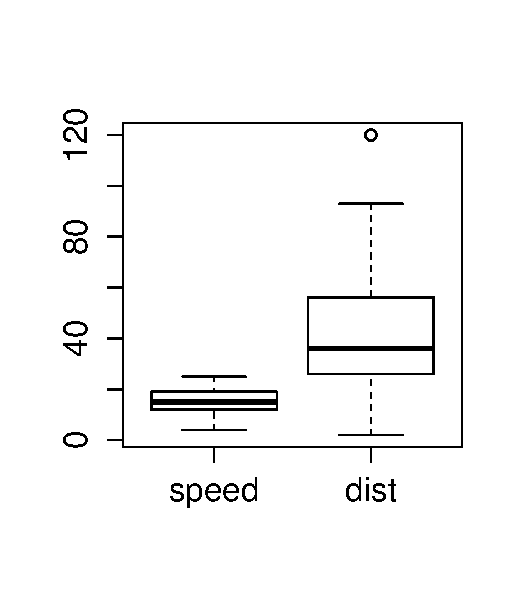
\includegraphics[width=6cm]{boxplot} % without file extension
\caption{This shows a boxplot}\label{fig: boxplot}
\end{figure} 

\section{Tables}

\subsection{Simple table}
\begin{tabular}{|c|c|}
\hline 
1 & 1 \\ 
\hline 
2 & 1 \\ 
\hline 
\end{tabular} 

\subsection{Proper table}
\begin{table*}\label{Table: Fit types}
  \centering
  \begin{tabular}{l@{\hspace{0.2cm}}l@{\hspace{0.2cm}}l} \toprule
  \textsc{Case} & \textsc{Explanation} & \textsc{Dimensions} \\ \midrule \addlinespace[0.2cm] 
  \multicolumn{3}{l}{Parameterization to virtual data, 3 PFTs:}  \\
  $V1$ & Data: SDD, GRO, reduced parameters &  $12,96$ \\ 
  $V2$ & Data: SDD, GRO, full parameters &  $26,96$  \\ 
  $V3$ & Data: SDD, reduced parameters &  $12,48$ \\ 
  $V4$ & Data: total SDD, reduced parameters &  $12,16$ \\ 
  $V5$ & Data: BM, reduced parameters &  $12,3$ \\  [0.2cm] 

  \multicolumn{3}{l}{Parameterization to Ecuadorian field data, 7 PFTs:} \\
  $E1$ & Data: SSD  &  $18,112$ \\ \bottomrule \\
\end{tabular}
\caption{Table caption}
\end{table*}

\end{document}
\end{lstlisting}



\chapter{References in \LaTeX}

In every scientific article it is important to clearly state your sources. You need to cite within your article and list all sources used at the end in your bibliography. 
Basically, there are two options to use references in \LaTeX. The first is to include references in the \LaTeX\ file directly, the second is to maintain an external file with references in the BibTeX format. For most cases, the latter will be preferred. There are few reasons to keep references directly in the \LaTeX\ file. One reason could be that a journal requires the submission in one \LaTeX\ file only (but in most cases you are allowed to include a .bbl file, which is created by BibTeX). In the following, we focus on the link to the BibTeX format. 

An excellent program to build your BibTeX database is Jabref, a free, open-source literature manager, which uses the BibTeX file format. As it is written in Java and distributed as a jar file, you can use it on any operating system with a Java Virtual Machine (JVM) installed. It is the first choice for everyone who works with \LaTeX, but it can also be used to insert citations in LibreOffice Writer or Microsoft Word\marginnote{Comprehensive information on how to link your Jabref database with Microsoft Word can be found at: \href{http://www.medicalnerds.com/how-to-use-jabrefbibtex-with-microsoft-word-2003/}{http://www.medicalnerds.com/how-to-use-jabrefbibtex-with-microsoft-word-2003/}}. 

This is an example of how an entry in your BibTeX database could look like:
\begin{lstlisting}[language=BibTeX]
@ARTICLE{Ovaskainen-Spaceandstochasticity-2006,
author = {Ovaskainen, O. and Cornell, S. J.},
title = {Space and stochasticity in population 
dynamics},
journal = {PNAS},
year = {2006},
volume = {103},
pages = {12781--12786},
number = {34},
month = aug,
}
\end{lstlisting} 
You will almost never have to type this yourself into your literature database in Jabref. Here are some examples of how to automatically import BibTeX entries from (1) journals, (2) databases (google scholar, ISI, \ldots) or even (3) package citations from \textsf{R}:
\begin{enumerate}
	\item Importing BibTeX entries from journal websites is highly recommended, since these are most likely to be correct. Instead of directly reading the paper (pdf) you may search for an ``export citation" button or similar on the journal website. After clicking on it, several format options should be provided. If you drag-and-drop the source to Jabref, it does not matter which format you choose (Jabref can handle it). If you use the import menu option in Jabref, choose the BibTeX format.
	\item Faster, but with higher risk of misspelling or other mistakes is the citation export directly from: 
	\begin{enumerate}[label=(\alph*)]
		\item \textbf{Google Scholar:} Click on ``cite" below the respective Google Scholar entry. At the bottom of the pop-up window you may choose the source format (see above).
		\item \textbf{ISI Web of Knowledge:} Tick the box on the left of the article you want to cite and choose from the drop-down list at the top of the page ``Save to EndNote desktop". A window pops up asking you to choose the contents to record. \marginnote{The default notepad on windows does not let you drag-and-drop. Use \href{https://notepad-plus-plus.org/}{notepad++} instead.} Hit send and open the output with an editor. From there drag-and-drop the source into jabref.
	\end{enumerate} 
\item If you want to cite \textsf{R} or an \textsf{R}-package, you may obtain the BibTeX source directly from R. For citing the base \textsf{R} program simply type \textsf{citation()} in the R console and hit Enter. If you wish to cite a specific package, e.g. \textsf{MASS}, the command to use is: \textsf{citation(``MASS")}. Copy the source from the \textsf{R} console to jabref.
\end{enumerate}

%For this purpose \LaTeX provides you with a link to the BibTeX format. 
Now that you have set up a BibTeX database, you can easily include it in your document and link to the entries in your .bib file. As with the inclusion of graphics, you can either put your .bib file in the same directory as the \LaTeX\ file and just refer to the .bib file by its name or put the .bib file elsewhere, but then you need to specify the whole path. You can include a database in your \LaTeX\ document by using the command \verb!\bibliography{}! at the end of your document, with the name of your database in curly brackets. The style of your bibliography is determined by the \verb!\bibliographystyle{}! command before the \verb!\bibliography{}! command, with the name of the style file in curly brackets. Here we use the \emph{chicago} citation style. To produce a pdf with all citations and the complete bibliography, you need to compile BibteX as well as \LaTeX\ at least two times.
% This process is still slightly faulty and it might require more compilation attempts until everything works properly.
Also make sure you are using the correct file encoding (e.g. UTF-8). Once everything is set, you can reference your sources within your document using the \verb!\citep{}! and \verb!\cite{}! commands from the \emph{natbib} package. The classical citation command is \verb!\citep{}!. It leads to your cited source enclosed in brackets while \verb!\cite{}! and \verb!\citet{}! only put the date of the citation in brackets allowing for an in-text citation. Once you cite a source in your document it will be listed in your bibliography as well. In this tutorial it is the last step but it is generally advisable to set up your bibliography at the beginning for your project to make citing fluent and to avoid mistakes. Now add a chapter about citations to your document and after that add your bibliography. A literature database is supplied in your training material. To make your citations look nicer and allow for more options include the \emph{natbib} package in your document. You can adjust the punctuation of your references by using the \verb!\bibpunct! command in your preamble. After including the \emph{natbib} package add the following line:\\
\verb!\bibpunct{(}{)}{;}{a}{}{,}!
\noindent Now everything is set for you to compile your document and have a look at your citations and your bibliography. Your \LaTeX\ file should now look like this:



\begin{lstlisting}

% This is my first Latex document. There are many documents like it, but this one is mine.

\documentclass{article}

\usepackage{graphicx}

\usepackage{multicol}              
\usepackage{multirow}
\usepackage{booktabs} 


\usepackage{natbib}
\bibpunct{(}{)}{;}{a}{}{,}  

\usepackage[]{hyperref}
\usepackage{color}
\usepackage{xcolor}
\definecolor{darkblue}{rgb}{0,0,.5}
\hypersetup{colorlinks=true, breaklinks=true, 
linkcolor=darkblue, menucolor=darkblue, 
urlcolor=darkblue, citecolor=darkblue}

\author{FirstName LastName}
\title{My first \LaTeX\ document}

\begin{document}
\maketitle

\begin{abstract}
This is my first \LaTeX! document. I am going to learn a lot about typesetting and writing articles in \LaTeX! and my papers will look really nice from now on.
\end{abstract}

\section{Introduction}
This is my \textbf{first} \emph{sentence}.

This is my \textit{second} sentence.

This is my third sentence. You can also put some distance between lines.\\[3mm]
Test 

\section{Doing equations} \label{equations}

\subsection{Inline equations}
This is our first inline equation $\alpha = 3.5$. $\lambda = \sqrt{\alpha}$. 

\subsection{Numbered equations}
This is our first numbered equation.

\begin{equation} \label{eq: definition of m}
m = \left( \frac{a \cdot b}{c} \right)
\end{equation}
 
This is our second numbered equation.
 
\begin{equation} \label{eq: definition of lambda}
\lambda = \int_{m_0}^\infty f(\Theta) d \Theta 
\end{equation}!.\\

\section{Labels and referencing}

In LaTeX, everything can be labeled, and after that it can be referenced. Consider for example section~\ref{sec: equations}, where eq.~\ref{eq: definition of lambda} and eq.~\ref{eq: definition of m} are defined.

\section{Including figures}

\begin{figure}
\centering
\includegraphics[width=6cm]{einstein} % without file extension
\caption{This shows Einstein in his study}\label{fig: einstein}
\end{figure}  

\begin{figure}
\centering
\includegraphics[width=3cm]{einstein}
\includegraphics[width=3cm]{einstein}
\caption{This shows Einstein in his study}\label{fig: einstein2}
\end{figure}  


\begin{figure}
\centering
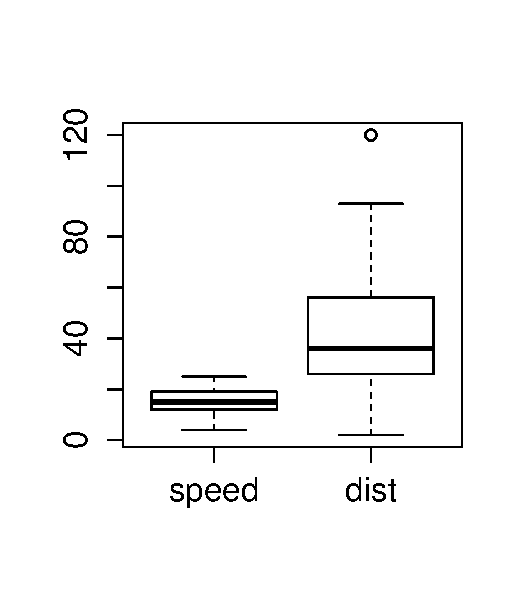
\includegraphics[width=6cm]{boxplot} % without file extension
\caption{This shows a boxplot}\label{fig: boxplot}
\end{figure} 

\section{Tables}

\subsection{Simple table}
\begin{tabular}{|c|c|}
\hline 
1 & 1 \\ 
\hline 
2 & 1 \\ 
\hline 
\end{tabular} 

\subsection{Proper table}
\begin{table*}\label{Table: Fit types}
  \centering
  \begin{tabular}{l@{\hspace{0.2cm}}l@{\hspace{0.2cm}}l} \toprule
  \textsc{Case} & \textsc{Explanation} & \textsc{Dimensions} \\ \midrule \addlinespace[0.2cm] 
  \multicolumn{3}{l}{Parameterization to virtual data, 3 PFTs:}  \\
  $V1$ & Data: SDD, GRO, reduced parameters &  $12,96$ \\ 
  $V2$ & Data: SDD, GRO, full parameters &  $26,96$  \\ 
  $V3$ & Data: SDD, reduced parameters &  $12,48$ \\ 
  $V4$ & Data: total SDD, reduced parameters &  $12,16$ \\ 
  $V5$ & Data: BM, reduced parameters &  $12,3$ \\  [0.2cm] 

  \multicolumn{3}{l}{Parameterization to Ecuadorian field data, 7 PFTs:} \\
  $E1$ & Data: SSD  &  $18,112$ \\ \bottomrule \\
\end{tabular}
\caption{Table caption}
\end{table*}

\section{References}

Referenced are extremely important \citep[see also][for more references]{Gintis-Costlysignalingand-2001,Archetti-Economicgametheory-2011}. However \citet{Cooper-CommunicationInCoordination-1992} note that this is not the case. 

\bibliographystyle{chicago} 

\bibliography{yourbibtexfile}

\end{document}
\end{lstlisting}


\chapter{Going further}

While expanding your document or when creating a new one you will probably get to a point where you want to do something that has not been covered by this tutorial. Here are three options how to find additional information and help:\\
\begin{itemize}
	\item The first\marginnote{When you encounter problems with \LaTeX\ search engines and forums are your best friends!} thing to do is to search for a solution on the web. \LaTeX\ has a very active community and most of the things you want to do will have already been done by someone and posted in some forum or wiki.
	\item Secondly, you can find so called "cheat sheets" (just search for them online) these are short scripts which list most of the functions and commands with a short explanation about what they do and how they are used.
	\item Finally, I provide some information on a list of useful packages in the \hyperref[appendix]{appendix} of this document.
	
\end{itemize} 

\makeatletter\@openrightfalse

\begin{appendices}



\chapter{FAQ}
\section*{\bfseries Q: Why does the referencing not work in my document?}
\subsection*{A$_1$: The path to your reference file is not correct:}
We recommend the use of relative file paths, such that your project folder contains different folders for different files, such as your .tex document (e.g. in a folder called ``thesis") and your .bib literature database (e.g. in a folder called ``literature"). If you use such a structure you may set \verb!\bibliography{../literature/yourbibtexfile}! at the end of your .tex document in order to link your .tex document with your .bib database.

Another option is to store all files in only one folder. Then you only need to set \verb!\bibliography{yourbibtexfile}! at the end of the .tex document. If you have many additional files, such as figures, this is not recommended.

There is one other option, which works as long as you are only working on one computer: The use of full file paths. This may look like this: \verb!\bibliography{C:/Users/User/documents/literature/yourbibtexfile}!, or the path to wherever yourbibtexfile.bib is stored. The obvious problem is that this specific file path must exist.

\subsection*{A$_2$: You mistakenly provided the file extension:}
In \verb!\bibliography{}! you must give the file name of your database without the extension (e.g. .bib). This means it must be \verb!\bibliography{yourbibtexfile}! instead of \verb!\bibliography{yourbibtexfile.bib}!

\subsection*{A$_3$: You need to do a LaTeX--BibTeX--LaTeX--LaTeX sequence:}
When compiling your .tex document the first time after adding a link to your literature database (.bib) you need to compile in LaTeX (F1 or F6), then in BibTeX (F8 or F11), and then twice in LaTeX again. 
This is necessary because each step produces auxiliary files that the next step uses. The first compiling in LaTeX generates an .aux file, which the citations need. The BibTeX compiling generates a .bbl file. The third compiling incorporates these references into the document, and the fourth is necessary to ensure that the insertion of these references still produces correct formatting.

\section*{\bfseries Q: Why are my figures or tables showing up in the wrong place?}
\subsection*{A: Figures and tables are placed in floats:}
In \LaTeX~ figures and tables are positioned in the text always following the same principles or rules (if not specified differently). To do this figures and tables are put into containers called floats. These also prevent the container items to be broken over pages. 

Now, the answer to this question may seem a bit circumventive: Simply don't care about the positioning of your tables and figures. If you finished your document and you still don't like the arrangement check \href{https://en.wikibooks.org/wiki/LaTeX/Floats,_Figures_and_Captions}{this} out. 



\chapter{Useful packages}

\label{appendix}
\noindent \textbf{This is a selection of packages, which may help you with everyday \LaTeX\ problems:}

\section{Encoding - inputenc}
The inputenc package allows for extended character encoding -- in particular for characters like \"A, \"U, etc..
\begin{lstlisting}
\usepackage[latin1]{inputenc}
\end{lstlisting}

\section{Typesetting - fontenc}
Extends the standard font family of \LaTeX\ to allow special characters.
\begin{lstlisting}
\usepackage[T1]{fontenc}
\end{lstlisting}

\section{Language specific labels and hyphenation - babel}
The babel package changes the standard labels of LaTeX like e.g. "`Table of Contents"´ or "`References"´ to the specified language. It also changes the hyphenation.
\begin{lstlisting}
\usepackage[ngerman]{babel}
\end{lstlisting}

\section{Including pdfs in your text - pdfpages}
The pdfpages package allows you to include pdf documents (e.g. a paper) in your document.
\begin{description}
	\item[Documentation] \href{http://www.ctan.org/tex-archive/macros/latex/contrib/pdfpages/pdfpages.pdf}{here}
	\item[Conflicts/Issues] Works only with pdflatex
\end{description}    

\section{Proper appendices - the appendix package}
The appendix package adds some useful features, which you will probably need when writing an appendix. It defines a appendices as new environment
\begin{lstlisting}
\usepackage[toc,page]{appendix}
...
\begin{appendices}
...
\end{appendices}
\end{lstlisting}
It is also possible to include subappendices within a section in the document
\begin{lstlisting}
\usepackage{appendix}
...
\section{Some stuff}
...
\begin{subappendices}
\subsection{Some boring stuff}
...
\end{subappendices}
\section{Some new stuff}
...
\end{lstlisting}

\section{For Formulae: Amsmath, amsfonts and amssymb}
The standard packages for extended mathematical symbols. Careful though, there is a conflict with the lineno package!
\begin{lstlisting}
\usepackage{amsmath, amsfonts, amssymb}
\end{lstlisting}
\begin{description}
	\item[Documentation] \href{http://www.ams.org/tex/amslatex.html}{here}
	\item[Conflicts/Issues] Conflict with the lineno package!
\end{description} 

\section{The color package}
Enables colors in \LaTeX.
\section{The xcolor package}
Extends color commands in latex. Enables in particular mixing of colors and provides some predefined colors.


\section{Underline - the ulem package}
Surprisingly, \LaTeX\ does not include an option for underlining text by default. This can be resolved using the \emph{ulem} package. Ulem replaces italics with underlining in emphasized text given by \emph{em} or  \emph{emph}. I recommend to use it with the \emph{normalem} option, which restores the normal \emph{em} behavior.
\begin{lstlisting}
\usepackage[normalem]{ulem}
...
\uline{Underlinded text}
\end{lstlisting}
%results in: \uline{Underlinded text}

\section{Spacing with setspace and linespread}
Many journals demand double spaced text for submission. 
\begin{lstlisting}
\usepackage{setspace}   
\end{lstlisting}
Double spacing can be activated by 
\begin{lstlisting}
\doublespacing   
\end{lstlisting}
A number of other spacing options is available and can be found in the manual. However, one drawback is that setspace does not change the spacing in the footnotes and floating environments like figures captions, tables etc. If double spacing is required throughout all text, tables etc. the best option is to use the linespread command 
\begin{lstlisting}
\linespread{1.6}
\end{lstlisting}
Note that although you want to have double spacing, the multiplication factor is 1.6, due to the way \LaTeX\ measures the spacing.

\section{Hyphenation}
To switch off hyphenation, use the hyphenat package. Careful: this will sometimes cause text to cross the border of your text box
\begin{lstlisting}
\usepackage[none]{hyphenat} 
\end{lstlisting}

\section{The preprint bundle}
Preprint is a bundle of packages which helps submitting preprints to journals. The most important package inside preprint is "`figcaps"´, which is described in the next section. The package is quite old, but the MPI for solar seems to use the package and has made some changes which may be interesting to modify for your own purposes, too. Find their website at:
\href{http://www.mps.mpg.de/software/latex/localtex/localltx.html#preprint}{preprint}

\section{figcaps}
Figcaps is part of the preprint bundle. It puts all tables, figure captions, and (optional) figures at the end of the document on separate pages.
\begin{lstlisting}
\usepackage[]{figcaps}
\end{lstlisting}
Figcaps has sometimes problems with the references to figure captions, which results in ?? when you refer to a figure number in your text. Put the code below somewhere after the \verb!\usepackage{figcaps}! command. This should resolve the problem (code from \href{http://www.pkblogs.com/phaseportrait/search/label/latex}{Ted Pavlic's blog}).
\begin{lstlisting}[]

\makeatletter
% This lets figcaps work with \ref
% However, forces \label outside of \caption
\def\phantomsection{\relax}
\let\oldfigurepage\@figurepage
\def\@figurepage{%
\@ifundefined{tf@pof}{}{%
\let\oldlabel\label%
\let\oldinput\@input%
\def\@input{\def\label{\oldlabel}\oldinput}%
\phantomsection%
\addcontentsline{toc}{section}{\figurepagename}}%
\oldfigurepage%
}
\let\@makefcaption\@makecaption
\let\oldtablepage\@tablepage
\def\@tablepage{%
\@ifundefined{tf@pot}{}{%
\clearpage%
\phantomsection%
\addcontentsline{toc}{section}{\tablepagename}}%
\oldtablepage%
}
\makeatother
\end{lstlisting}
\end{appendices}

\end{document}
